\section{Physical problems}
WTR's problems are not limited to its rear wheels.
The front wheels have their share of problems as well.

\subsection{Loose Batteries}
Generally speaking, when something goes wrong electrically, it is because a wire has come loose.
WTR has a different problem, which is illustrated in figure ~\ref{fig::batteries}.

\begin{figure}[H]
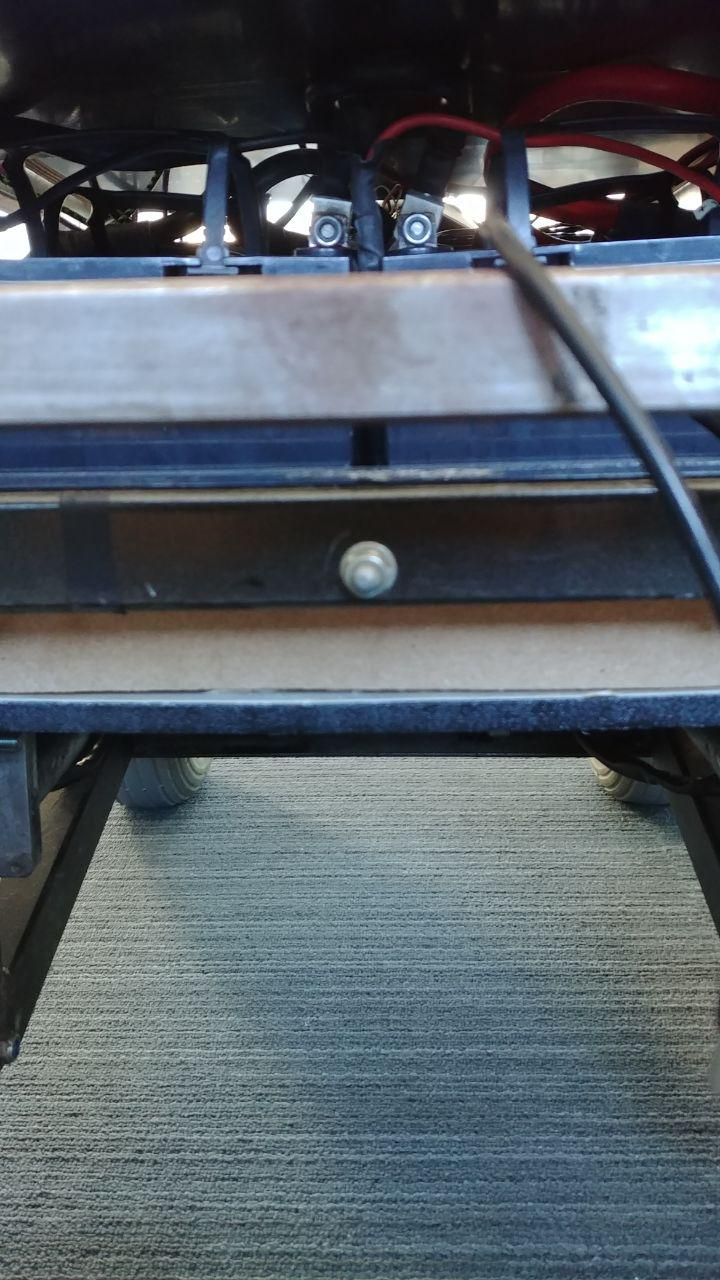
\includegraphics[width=8cm]{batteries.jpg}
\caption{As is slightly visible, the wooden plank is bending}
\label{fig::batteries}
\end{figure}

The wooden plank the batteries are resting on is bending, and the glue/tape which was used to attach that plank is letting go.
While the current situation is not immediately concerning, if WTR were to hit a bump and the force of all the batteries were to hit the plank at once it could snap off of break in two.
That would be a lot of clean-up and work for the group.

Another issue is that the batteries don't have a proper mount, so nothing really keeps them from sliding about.
This means a shifting weight within WTR, which is detrimental to the accuracy of its driving.

\subsubsection{solutions}
These issues are easy enough to resolve.
For the first issue, a metal L-joint around the center of the plank would reinforce the structure so that the bottom falling out would become much less likely.

The second issue can be resolved easily (though not very neatly) by simply wedging some wood or spare non-conductive material between the batteries to keep them from shifting around.
The neater but more time and effort consuming method would be to create a frame that goes over the batteries keeping them in place.


\subsection{After Effects of Collisions}
WTR is getting along in its age.
This is the 4th year of its life, and as such it has had to deal with a fair few knocks and scrapes.
One such collision ended up knocking one of the front wheels so that it was stuck at an angle.
As a result, the wheel kept scraping against the frame, and the effects can still be seen in figure ~\ref{fig::wheelclip}

\begin{figure}[H]
\centering
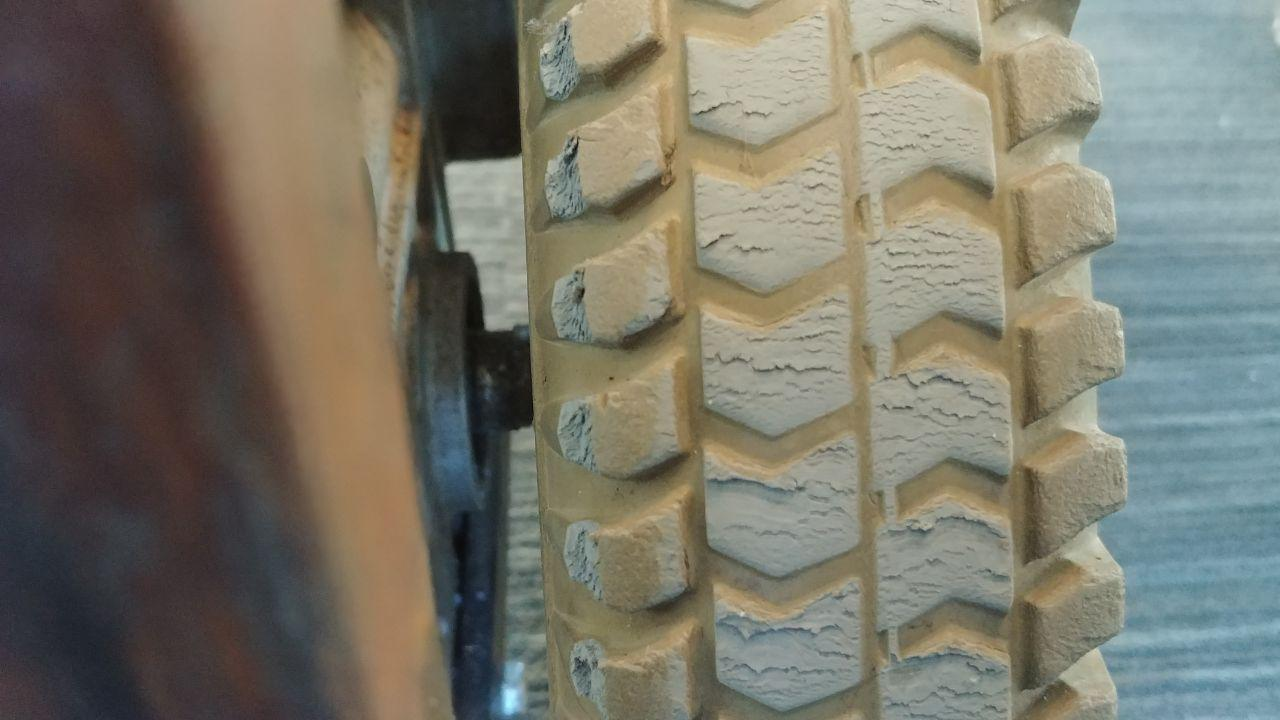
\includegraphics[width=12cm]{clippedwheel.jpg}
\label{fig::wheelclip}
\caption{The left side of the wheel shows the damage done by the frame.}
\end{figure}

Another issue which can be seen on figure ~\ref{fig::wheelclip} is that the tread on the tires is being worn away.
This results in the wheels slipping on the floors of Windesheim, which are mostly smooth, where they are not carpeted.
Since the two wheels are at different levels of wear due to the aforementioned grinding of the tire against the frame, they slip different amounts.
This unfortunately means that the accuracy of any soft-ware based solutions will be lessened.

\subsubsection{Solutions}
The effects mentioned above can be counteracted.
When it comes to the clipping issue on the left front tire, it has already been resolved by straightening out the axle and increasing the rigidity of the suspension, causing WTR to stand a little taller and putting a bit of distance between the tire and the frame.

The issue of slipping is not as easy to resolve.
New tires would be a lot of trouble to acquire and replace, and would at best be a stop-gap measure.
Because WTR is so heavy, even without the cover, the tires would get worn down quickly anyway.
The best solution therefore is to either lighten WTR, or attempt to reduce the impact of the slipping.

By adding rotary encoders, the amount of rotations made by both wheels can be tracked, so if one tire keeps slipping, the other can reduce its speed to compensate for the turn that would be caused by the different speeds of both sides of WTR.





\newpage